\documentclass[main]{subfiles}
\begin{document}

%@@@@@@@@@@@@@@@@@@@@@@@@@@@@@@
% Main Topics: consequences of projections, Farkas Lemma, standard form
% polyhedra, cones
% author: Vanessa Leite

\section{Farkas Lemma and Standard Form Polyhedra}

\subsection{Some consequences from lecture 4}

\paragraph{Corollary: If I take a polyhedron $P = \{ x \in \mathbb{R}^n \mid Ax
\leq b\}$, the projection $proj_{(x_1, \dots, x_i}(P)$ is a polyhedron (by
removing points). }

\paragraph{Corollary: Take a polyhedron $P = \{ x \in \mathbb{R}^n \mid Ax \leq
b\}$, consider the set $Q$ (the set of all vectors of the form: $\{ wx \mid x
\in P \}$, where $w \in \mathbb{Q}^{d \times n}$; $wx \subseteq \mathbb{R}^d$.
$Q$ is a polyhedron.}

\subparagraph{Proof:}
Let's define another set $D = \{(x,y): wx - y = 0$, $x \in P\} = \{(x,y) \mid
wx -y = 0$, $Ax \leq b\} \subseteq \mathbb{R}^{n+d}$. $Q$ is the projection of
$D$ on the space of $Q = proj_y (D) = \{ y \in \mathbb{R}^d \mid \exists x \in
\mathbb{R}^{d \times n}$ such that $\underbrace{(x,y) \in D}_{\text{that means
$wx =y$}} \}$.

\paragraph{Corollary: Let $x^1, \dots, x^t \in \mathbb{Q}^n$ (set of vectors).
$conv(x^1, \dots, x^t)$ is a polyhedron.}

\paragraph{Corollary: Let $x^1, \dots, x^t \in \mathbb{Q}^n$ (set of vectors). 
$cone(x^1, \dots, x^t)$ is a polyhedron.}

\begin{figure}[!h]
  \label{fig:projection}
  \centering
    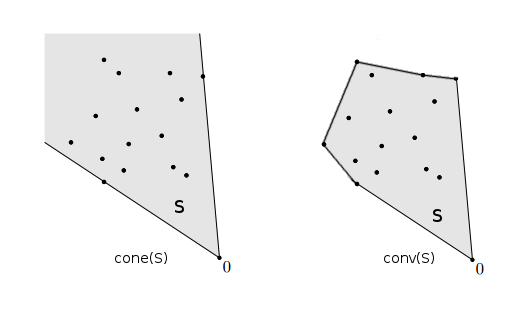
\includegraphics{imgs/conv-cone.png}
\end{figure}

Define a matrix $X =[x^1 \mid x^2 \mid \dots \mid x^t] \in
\mathbb{Q}^{n \times t}$.

\subparagraph{Proof: convex hull}
$conv(x^1, \dots, x^t) = \{ \sum_{i=1}^{t} \lambda_i x^i \mid \lambda_i \geq 0
\forall i, \sum_{i=1}^t \lambda_i = 1 \}$.

$ = \{ X \times \lambda \mid \lambda \in \mathbb{R}^t_+$, $\lambda_i \geq 0$, 
$\mathds{1}^T \lambda = 1 \} \rightarrow $ is a polyhedron from the previous
corollary.

\subparagraph{Proof: cone}
Cone is unbounded and with a finite many rational vectors, a rational cone is a 
polyhedron.
$cone(x^1, \dots, x^t) = \{ \sum_{i=1}^{t} \lambda_i x^i \mid \lambda_i \geq 0
\forall i \}$.
$ = \{ X \times \lambda \mid \lambda \in \mathbb{R}^t_+$, $\lambda_i \geq 0 \}
\rightarrow $ is a polyhedron from the previous corollary.

\paragraph{Corollary: Take a polyhedron $P \subseteq \mathbb{R}^n$. Then $P
\neq \emptyset \iff proj_{(x_1, \dots, x_{n-1})}(P) \neq \emptyset$}

\paragraph{Theorem - Farka's Lemma: Either $Ax \leq b, x \in \mathbb{R}^n$ has
a solution or $y^T A = 0, y^T b < 0, y \geq 0$ has a solution. Both are
exclusive. If $y^T A = 0$ and $y^T b < 0, y \geq 0$ then $Ax \leq b, x \in
\mathbb{R}^n$ is empty.}

\subparagraph{Proof - do not exist simultaneously $x$ and $y$ such that both 
systems ae feasible}

Suppose this is not true, then $\underbrace{y^T Ax}_{=0}
\underbrace{\leq}_{y \geq 0} y^T b \rightarrow 0 \leq y^T b < 0$. 

Let $P = \{x \in \mathbb{R}^n \mid Ax \leq b \}$. For $L \in \{1, \dots, n \}$,
let $C^{(i)} = \{ y \geq 0 \mid y^T A_{\cdot k} = 0, \forall k \geq n-i+1 \}$.

$P^{(i)} = proj_{(x_1, \dots, x_{n-i})}(P) = \{ \bar{x} \in \mathbb{R}^{n-i}
\mid \sum_{k=1}^{n-i}y^T A_{\cdot k} \bar{x}_k \leq y^T b \forall y \in C^{(i)}
\}$.

Then $C^{(n)} = \{y \geq 0 \mid y^T A = 0 \}$, $P^{(n)} = \{0 \leq y^Tb
\forall y \in C^n \}$
$P \neq \emptyset \iff P^{(1)} \neq \emptyset \iff \dots \iff P^{(n)} \neq
\emptyset$.
Hence, either $P \neq \emptyset$ or $P = \emptyset \iff P^{(n)} = \emptyset
\iff \exists y \geq 0$ such that $y^T A = 0$ and $y^T b < 0$.

\subsection{Standard form polyhedra}
Definition: Take a matrix $A \in \mathbb{Q}^{m \times n}$ of full row rank. 
Then take a vector $b \in \mathbb{Q}^n$. A polyhedron of the type $\{x \in 
\mathbb{R}^n_+ \mid Ax = b \}$ is called in standard form.

\textbf{Observation:} $\{x\in \mathbb{R}^n_+ \mid Ax = b \}$ is a polyhedron.\\

A polyhedron of the form ($\{x \in \mathbb{R}^n \mid Ax \leq b \}$ can be
brought into standard form:

$Ax \leq b, x \in \mathbb{R}^n \rightarrow$ split into positive and negative 
i.e., For $x \in \mathbb{R}^n$ write $x = x^+ - x^-, x^+, x^- \geq 0$.

Artificially transform in equations by introducing slack variables (how far we
are from the plane): $A_{i\cdot} x \leq b_i \rightarrow A_{i\cdot}x + y_i =
b_i, y_i \geq 0$.

Then, we can represent $\{ x \in \mathbb{R}^n \mid Ax \leq b \}$ as $\{(x^+,
x^-, y) \in \mathbb{R}^{2n+m} \mid [A | -A | \underbrace{I}_{\text{for the
y's}}]\begin{pmatrix} x^+ \\ x^- \\ y \end{pmatrix} = b$, $x^+, x^-, y \geq 0
\}$.

\textbf{Observation: A polyhedron in standard form has no lines.}
$P = \{ x \in \mathbb{R}^n_+ \mid Ax = b \} \subseteq \mathbb{R}^n_+$.
\begin{itemize}
\item theorem from lecture 3 applies.
\item optima are characterized by extreme points, if the optima is finite.
\end{itemize}

\paragraph{Theorem: $Ax = b, x \geq 0$ has a solution iff $\forall y \in 
\mathbb{R}^n$ such that $y^T A \geq 0$ then $y^T b \geq 0$.}

\subparagraph{Proof}
\todo[inline]{proof as homework!}

\paragraph{Theorem: $x^* \in P = \{x \in \mathbb{R}^n_+ \mid Ax = b$
(polyhedron in standard form (= full row rank))$ \}$ is a basic feasible
solution iff there exists a basis $B \subseteq \{1, \dots, n\}$, $\abs{B}=m$
(number of constraints), with the properties:}
\begin{itemize}
\item $A_B \in \mathbb{R}^{m \times m}$ is invertible
\item $x^*_i = (A^{-1}_B b)_i$: $\forall i \in B$
\item $x^*_i = 0$, $\forall i \in N=\{1, \dots, n\}\setminus B$
\end{itemize}

\paragraph{Theorem: Let $v^1, \dots, v^t \in \mathbb{Z}^n$ be vectors and $y 
\in cone(v^1, \dots, v^t)$. There exists a subset $B \subseteq \{1, \dots, t\}
$, $\abs{B} \leq n$ and multipliers $\mu_i > 0 \forall i \in B$ such that $y = 
\sum_{i \in B} \mu_i v^i$}

\subparagraph{Proof:}
Consider $c^* = min \sum_{i=1}^{t} \lambda_i$, st $V \lambda = y, \lambda \geq
0$, $V = [v^1 | \dots | v^t ] \in \mathbb{Z}^{m \times t}$.
$Q = \{\lambda \in \mathbb{R}^t_+ \mid V \lambda = y \}$ is a standard form
polyhedron. From previous arguments, $c^* \geq 0 \rightarrow c^*$ is finite,
i.e., there exists extreme point $x^* \in Q$ attaining the optimum solution.
$\rightarrow \exists B \subseteq \{1, \dots, t \}, \abs{B}=n$, such that
$x^*_i = 0, \forall i \notin B$.

\paragraph{Theorem of separating hiperplane (consequence of Farka's Lemma): For
$v^1, \dots, v^t \in \mathbb{Z}^n$, let $b \in \mathbb{R}^n$. $b \in cone(v^1,
\dots, v^t)$ or $\exists c$ (a hiperplane) $\in \mathbb{R}^n$, such that $c^T
x\geq 0 \forall x \in cone(v^1, \dots, v^t)$ and $c^T b < 0$.}

\subparagraph{Proof:}
Let $V = [v^1, \dots, v^t] \in \mathbb{Z}^{n \times t}$. $b$ is not in the cone
($b \notin cone(v^1, \dots, v^t)$) iff our linear system ($V \lambda = b,
\lambda \geq 0$) has no solution.\\

Farka's lemma $\rightarrow \exists y \in \mathbb{R}^n$ such that $y^T V \geq 0, 
y^T b < 0$.\\
Define $c = y$.
\begin{itemize}
\item $c^T b = y^T b < 0$
\item $\forall x \in cone(v^1, \dots, v^t), x = V \lambda, \lambda \geq 0$
\end{itemize}

$c^T x = \underbrace{c^T V}_{\geq 0} \underbrace{\lambda}_{\geq 0} \geq 0$.

\end{document}